Matematický model, ktorý opisuje bioreaktor je nelineárny model. To znamená, že odozva systému je rôzna pre rovnakú veľkosť skokovej zmeny. Túto nelinearitu si možno všimnúť na Obr. \ref{fig:1}. Ďalej si môžme všimnúť prudký narást koncentrácie produktu na počiatku, ktorý bol spôsobený nadbytkom biomasy a malým množstvom substrátu v systéme. Po ustálení dynamika produtku pripomímna systém 1. rádu. Na druhej strane v dynamike tvorby biomasy sa prejavuje nestabilná nula (menšie podkmity), ktoré sú spôsobené veľkou časovou konštantou tvorby biomasy a malou časovou konštantou odtoku suspenzie. V dynamike substrátu sa zasa prejavuje stabilná nula, ktorá opäť súvisí s rýchlym prítokom česrstvého média a pomalšou spotrebou na tvorbu biomasy a produktu.

\begin{figure}[H]
% RP: Ja vacsinou tieto identifikatory umiestnenia floatov ``[H]'' ani nepouzivam. Latex vie najlepsie ako umiestnovat obrazky/tabulky aby vysledny dokument vyzeral dobre
	\centering
	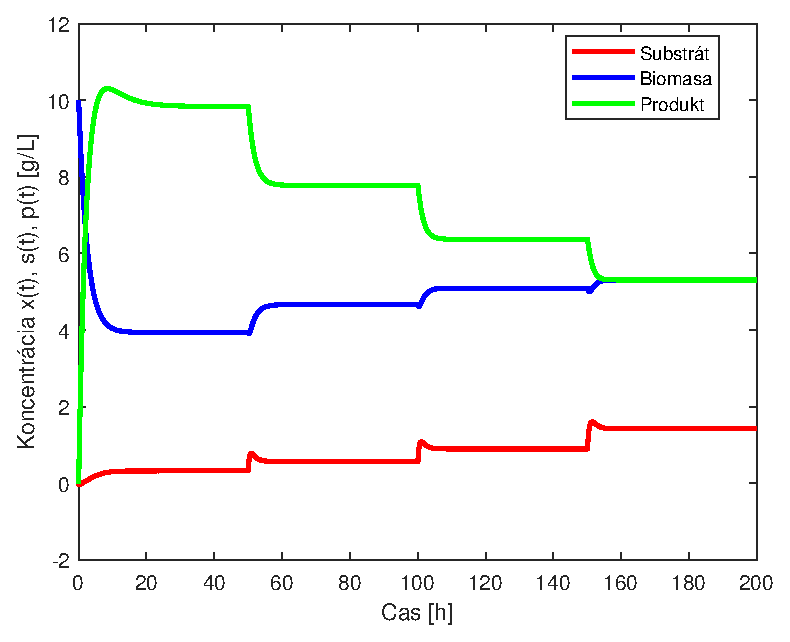
\includegraphics[width=1\linewidth]{images/step_change}
	% RP: Kvalita obrazku (aj dalsich) nie je nic moc. Zda sa mi, ze ma na okrajoch prilis vela bieleho miesta. Takisto je dost neostry. Neviem, aky sposob ukladania obrazkov z Matlabu pouzivate, ale skuste najst nejaky iny, resp. taky, ktory je vhodny pre pouzitie v Latexom generovanych dokumentoch. Internet urcite poradi. Ja to robi pomocou prikazu print, kde sa da stanovit priblizna velkost obrazku v samotnom dokumente a teda vysledok byva ostry. Hrubka ciar by mala byt aspon 2.
	\caption[]{Viacnásobná skoková zmena rýchlosti riedenia $D$ pri začiatočných podmienkach $p_0 = s_0 = 0, x_0 = 30 gL^{-1}$.}
	\label{fig:1}
\end{figure}

% Rp: ``Réžim'' -> ``Režim''
Réžim fungovania bioreaktora má významný vplyv na dynamiku celého systému a pri určitých podmienkach Monod model a model s inhibíciou môžu vykazovať rovnaké správanie, presne ako je tomu na Obr. \ref{fig:1}. Avšak, tieto modely sa odlišujú vo formulácii špecifickej rýchlosti rastu, ktorý má zásadný vplyv na dynamiku systému. Ako vidno na Obr. \ref{fig:2} pri Monod modely sa špecifická rýchlosť rastu limitne blíži ku maximálnej špecficikej rýchlosti rastu, zatiaľ čo model s inhibícou dosahuje svoje maximum v bode $S^{*} = \sqrt{K_M K_i}$. 

\begin{figure}[H]
	\centering
	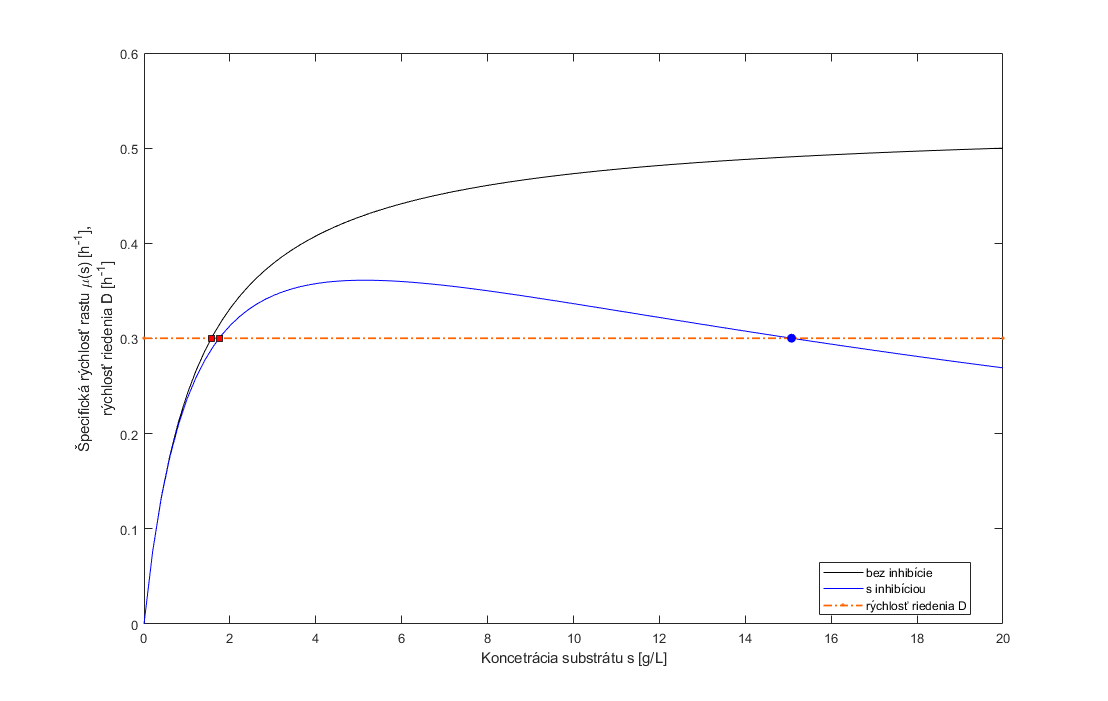
\includegraphics[width=1\linewidth]{images/spec_grow_rate_comparison}
	\caption[]{Porovnanie priebehu špecifickej rýchlosti rastu Monod modelu (červená) a modelu s inhibíciou (modrá). Červeným štvorčekom sú označené nenulové stabilné ustálené stavy, modrou guličkou je označený nestabilný stav.}
	\label{fig:2}
\end{figure}

\begin{figure}[H]
% RP: Tu uz na obrazkoch nie je vidiet skoro nic.
	\begin{subfigure}{.5\textwidth}
		\centering
		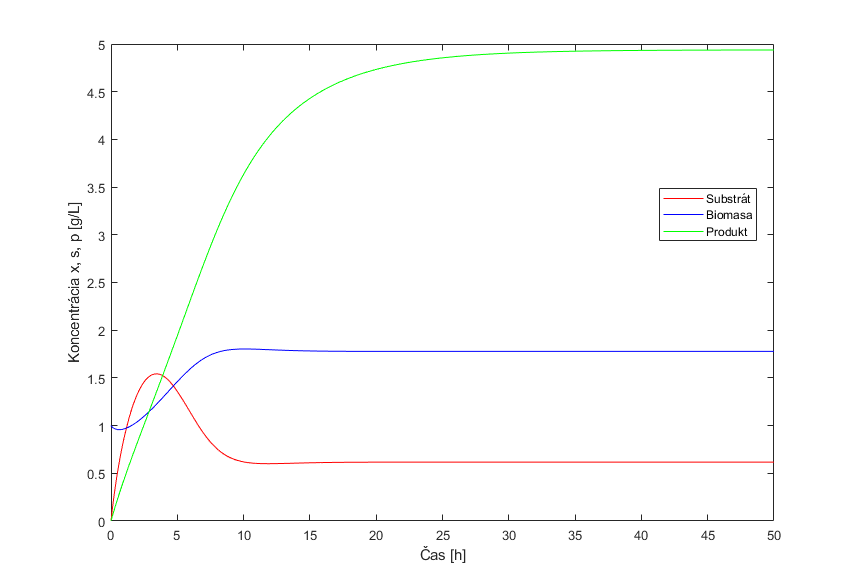
\includegraphics[width=1\linewidth]{images/dyn_wo_inhb}
		\caption[]{Monod model}
	\end{subfigure}
	\begin{subfigure}{.5\textwidth}
		\centering
		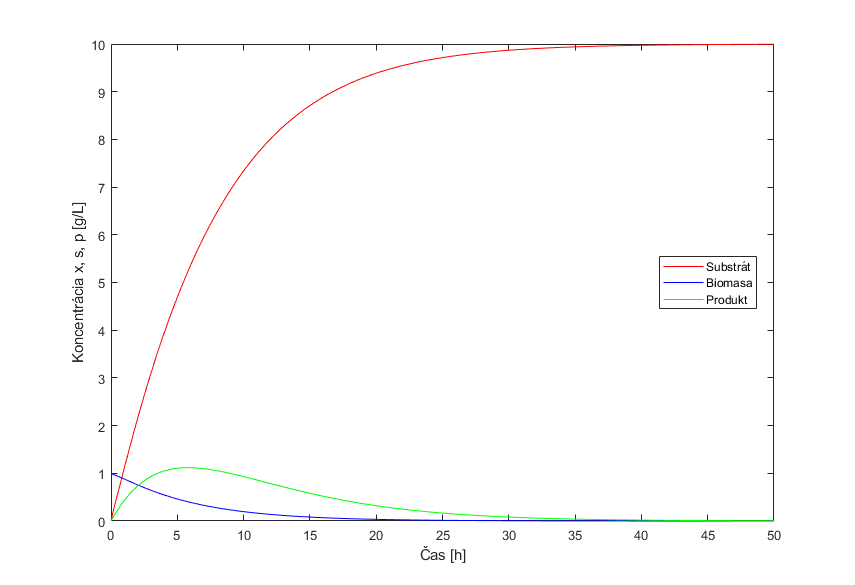
\includegraphics[width=1\linewidth]{images/dyn_inhb}
		\caption[]{Model s inhibíciou}
	\end{subfigure}
	\caption{Porovnanie dynamiky modelov pri rovnakých pracovných podmienkach.}
	\label{fig:3}
\end{figure}

\noindent Pri nesprávne zvolených pracovných podmienkach, či už počiatočných podmienkach systému, koncentrácie čerstvého substrátu alebo rýchlosti riedenia, model s inhibíciou bude vykazovať diametrálne odlišné správanie od Monod modelu, ako to je zobrazené na Obr. \ref{fig:3}.